%%%%%%%%%%%   Back Cover of the Book               %%%%%%%%%%%%%%%%%%%%%%%%%%%%%%%%%%%%%%%%%%%%%%%%%%%%%
\clearpage   
% Add a background image for the full page
\begin{tikzpicture}[remember picture,overlay]
\node[inner sep=0pt] at (current page.center) 
{\includegraphics[width=\paperwidth,height=\paperheight]{Ghats1860.jpg} };%  Repeat same block for another image
\end{tikzpicture}


%\noindent 
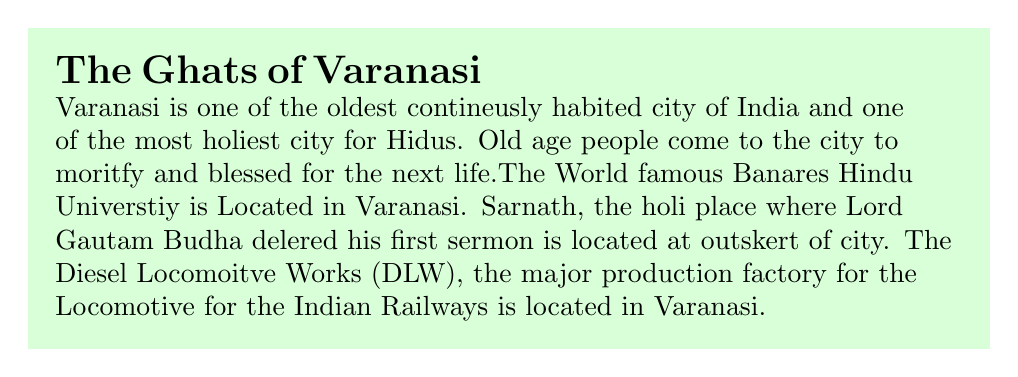
\begin{tikzpicture}     % Now typeset a sample box.
  \node[text width=.95\textwidth, fill=green!30, fill opacity=0.5, text opacity=1, inner sep=10pt]{
  {\bf\Large The Ghats of Varanasi } \\
  Varanasi is one of the oldest contineusly habited city of India and one of the most holiest city for Hidus. 
  Old age people come to the city to moritfy and blessed for the next life.The World famous Banares Hindu Universtiy is Located in Varanasi. 
  Sarnath, the holi place where Lord Gautam Budha delered his first sermon is located at outskert of city. 
  The Diesel Locomoitve Works (DLW), the major production factory for the Locomotive for the Indian Railways is located in Varanasi.
};
\end{tikzpicture}


\vspace*{\stretch{1}}


\begin{center}
\colorbox{white}{\EANisbn[SC4]}
\vspace*{\baselineskip}

\textbf{\textcolor{red!80}{Expotech Division \textbullet\ RITES Limited  \texttt{http://wwww.RITES.com}}}
\vspace*{\baselineskip}

\colorbox{white}{
\textbf{\textcolor{blue!60}{Ghats in Varanasi and Qutub Minar in Delhi  \textbullet\ idea: \texttt{gopalkumar@rites.comm}}}   }
\end{center}
